% 第二章 项目内容
\section{项目内容}

\subsection{项目界面}

\subsubsection{系统架构}

智舆系统采用\textbf{前后端分离、分层解耦}的现代化架构设计:

\begin{table}[H]
\centering
\caption{系统架构分层}
\begin{tabular}{L{3cm}L{7cm}L{2cm}}
\toprule
\textbf{层级} & \textbf{技术组件} & \textbf{状态} \\
\midrule
前端展示层 & Vue3 + Vite + 高德地图3D + Three.js + ECharts + Element Plus + TailwindCSS + Pinia + Socket.io & 已实现 \\
后端服务层 & FastAPI + Celery + Redis + WebSocket & 开发中 \\
AI分析层 & 讯飞星火4.0 + LangGraph多Agent + LoRA微调 + RAG & 开发中 \\
3D生成层 & Tripo AI / Meshy + 3D Gaussian Splatting + TripoSR & 规划中 \\
语音交互层 & 讯飞TTS + 讯飞ASR + 实时语音流式交互 & 规划中 \\
数据采集层 & MediaCrawler + Scrapy + Playwright + 官方API接口 & 规划中 \\
数据存储层 & PostgreSQL + Elasticsearch + MinIO + Chroma(向量库) & 规划中 \\
\bottomrule
\end{tabular}
\end{table}

\begin{figure}[H]
\centering
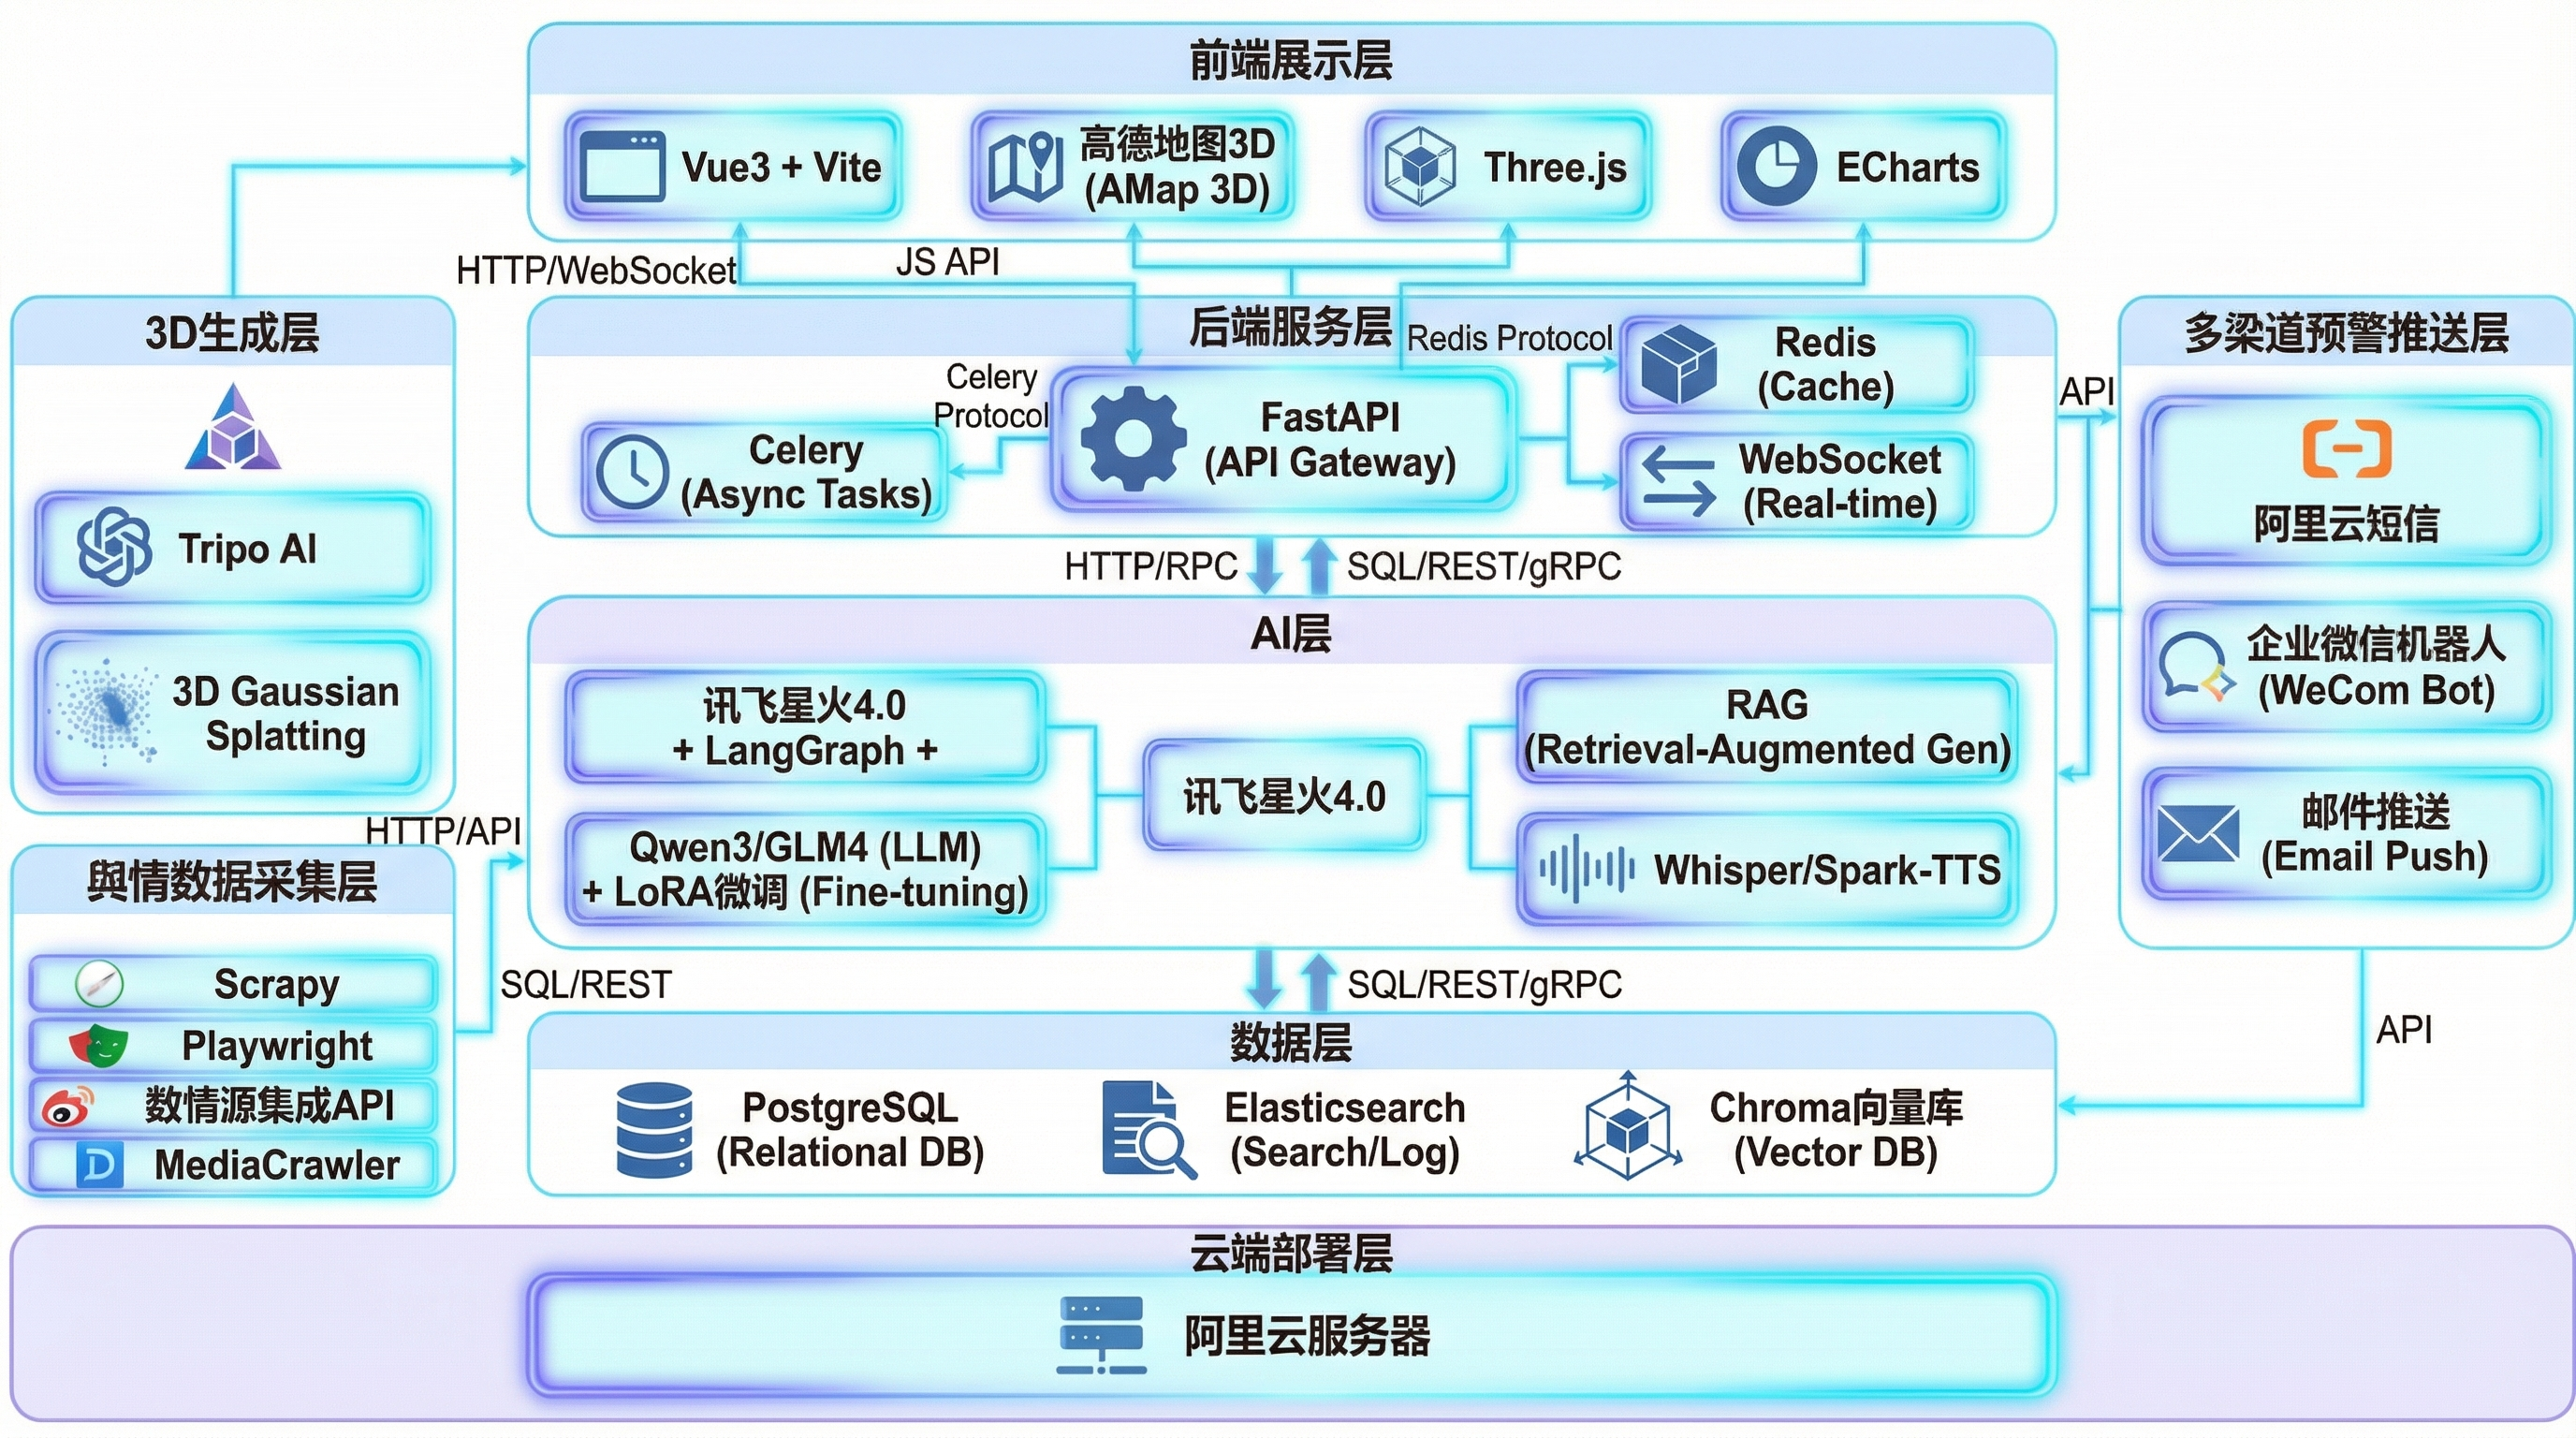
\includegraphics[width=0.85\textwidth]{../picture/fig04_architecture.png}
\caption{系统整体架构图}
\end{figure}

\subsubsection{功能模块}

系统包含\textbf{六大核心功能模块}:

\textbf{模块一:实时舆情监测} -- 多源数据采集,覆盖微博、抖音、小红书等主流平台;多模态解析;实时预警推送。

\begin{figure}[H]
\centering
\includegraphics[width=0.4\textwidth]{../source/UI/筛选界面.png}
\caption{实时舆情监测筛选界面}
\end{figure}

\textbf{模块二:智能舆情分析} -- 情感极性分析(准确率超90\%);主题聚类;传播路径追踪;影响力评估。

\begin{figure}[H]
\centering
\begin{subfigure}[b]{0.48\textwidth}
    \includegraphics[width=\textwidth]{picture/ui_ai_analysis.png}
    \caption{AI智能分析面板}
\end{subfigure}
\hfill
\begin{subfigure}[b]{0.48\textwidth}
    \includegraphics[width=\textwidth]{picture/ui_wordcloud.png}
    \caption{舆情关键词云}
\end{subfigure}
\caption{智能舆情分析模块界面}
\end{figure}

\textbf{模块三:3D地图可视化} -- 四级区域穿透(全国$\rightarrow$省份$\rightarrow$地级市$\rightarrow$县级);3D建筑高亮;热力图叠加;飞行动画。

\textbf{模块四:AI场景还原} -- 文字转3D;图片转3D;地图叠加。

\begin{figure}[H]
\centering
\includegraphics[width=0.85\textwidth]{../source/UI/3D建筑+场景还原.png}
\caption{3D建筑与场景还原界面}
\end{figure}

\textbf{模块五:走向预测与决策模拟} -- 趋势预测;多场景推演;决策建议;效果模拟。

\begin{figure}[H]
\centering
\begin{subfigure}[b]{0.48\textwidth}
    \includegraphics[width=\textwidth]{picture/ui_trend_analysis.png}
    \caption{舆情趋势预测}
\end{subfigure}
\hfill
\begin{subfigure}[b]{0.48\textwidth}
    \includegraphics[width=\textwidth]{picture/ui_decision_sim.png}
    \caption{决策模拟器}
\end{subfigure}
\caption{走向预测与决策模拟模块界面}
\end{figure}

\textbf{模块六:语音交互与播报} -- 语音预警;语音指令;智能问答。

\begin{figure}[H]
\centering
\includegraphics[width=0.75\textwidth]{../picture/fig05_modules.png}
\caption{六大功能模块关系图}
\end{figure}

\subsubsection{界面设计}

系统界面采用\textbf{赛博朋克+玻璃拟态(Glassmorphism)}设计风格:

\textbf{主界面布局}采用五区域设计。顶部\textbf{Dynamic Island导航栏}集成时间显示、功能图标快捷入口、智能搜索与系统设置,提供一站式操作入口。左侧\textbf{舆情监控筛选栏}支持按风险等级(高/中/低)、分类标签(交通/民生/消费/餐饮/环境)、时间范围(24小时/3天/7天/30天)进行多维度过滤,并实时展示舆情列表。中央\textbf{3D地图主视图}基于高德地图JS API 2.0实现三维城市可视化,支持区域边界霓虹渲染、舆情热点标注、关键词浮动展示等效果。右侧\textbf{智能分析面板}展示AI生成的情感分析结果、趋势预测曲线、舆情词云、决策模拟交互与结果展示。右下角\textbf{图层控制工具栏}提供热力图、边界线、3D建筑模型、悬浮标志、事件关联线等可视化图层的开关控制。

\textbf{视觉特色}:霓虹色彩(Cyan-400主色调)、毛玻璃半透明效果、动态光效与粒子、3D纵深空间感。

\textbf{响应式设计}:系统采用单一代码库,通过CSS媒体查询适配不同屏幕。Web/PC端(lg/xl)呈现完整三栏布局(侧边栏+核心地图+右侧面板),支持鼠标精细操作和复杂3D交互;移动端(xs/sm)采用单列布局,地图作为背景,侧边栏收起为汉堡菜单,功能面板转为底部抽屉(Bottom Sheet),触控区域经过优化以适配手指操作。

\textbf{用户交互流程}:系统引导用户完成从"发现问题"到"解决问题"的完整闭环,分为四个阶段。\textbf{感知阶段}:3D地图上某区域出现红色脉冲警报,左侧实时列表弹出"突发"标签的新闻条目,用户点击地图红点或列表条目触发下一阶段。\textbf{分析阶段}:地图视角自动平滑推拉至事发地点,右侧面板滑出事件详情卡片,展示AI生成的事件摘要、情绪占比分析,若可用则弹出3D现场还原全息影像。\textbf{预测阶段}:地图上显示动态箭头预示舆情可能扩散区域,趋势图展示未来24小时热度预测曲线,AI助手弹出决策建议。\textbf{模拟阶段}:用户打开决策模拟器,选择或输入决策方案,系统即时计算后地图警报区域根据模拟结果变化,趋势图生成虚线分支对比不同决策下的未来走向。

\begin{figure}[H]
\centering
\includegraphics[width=0.95\textwidth]{../source/UI/ui_main_interface.png}
\caption{系统主界面}
\end{figure}

\begin{figure}[H]
\centering
\makebox[\textwidth][c]{\includegraphics[width=1.3\textwidth]{../source/UI/ui_elements_guide.png}}
\caption{界面元素详解图}
\end{figure}

\begin{figure}[H]
\centering
\includegraphics[width=0.9\textwidth]{../picture/fig07_interaction_flow.png}
\caption{界面交互流程图}
\end{figure}

\subsection{项目特色}

\subsubsection{核心创新点}

\textbf{创新点一:AI驱动的舆情场景3D还原}

这是本项目最具创新性的功能。智舆系统创新性地引入\textbf{AI 3D生成技术},可根据舆情内容自动生成现场3D模型。

\textbf{技术实施路径}:首先,系统通过讯飞星火4.0大模型对舆情内容进行语义理解,提取关键场景元素(如"建筑物"、"车辆"、"人群"等),并根据事件类型生成结构化场景描述JSON。对于\textbf{文字舆情},系统将场景描述转换为Tripo AI可识别的Prompt,调用text-to-3D API生成模型,平均耗时约10秒。对于\textbf{图片舆情},采用TripoSR开源模型进行单图3D重建,该模型基于Transformer架构,支持本地部署,推理速度约500ms/张。对于\textbf{视频舆情},首先通过讯飞LFASR进行音频转写,提取视频关键帧进行3D重建,并将转写文本与3D场景融合,生成完整的可交互场景。生成的3D模型统一转换为GLTF格式,通过Three.js加载并叠加到高德地图GLCustomLayer上,实现\textbf{"在地图上看见新闻现场"}的沉浸式体验。

\begin{figure}[H]
\centering
\includegraphics[width=0.9\textwidth]{../picture/fig08_ai_3d_workflow.png}
\caption{AI 3D场景还原技术流程图}
\end{figure}

\textbf{创新点二:多Agent协作的决策模拟系统}

基于\textbf{LangGraph}框架构建多Agent协作体系:

\begin{table}[H]
\centering
\caption{多Agent协作体系}
\begin{tabular}{L{2.5cm}L{3cm}L{3.5cm}L{4cm}}
\toprule
\textbf{Agent} & \textbf{职责} & \textbf{输入} & \textbf{输出} \\
\midrule
分析Agent & 舆情深度分析 & 原始舆情数据 & 情感、主题、影响力分析 \\
预测Agent & 走向趋势预测 & 分析结果+历史数据 & 乐观/中性/悲观场景 \\
决策Agent & 生成应对方案 & 预测结果 & 多套决策建议 \\
模拟Agent & 模拟执行效果 & 用户选择的决策 & 效果评估报告 \\
\bottomrule
\end{tabular}
\end{table}

\textbf{技术实施路径}:LangGraph采用有向图结构管理Agent状态流转,系统状态定义为$S = \{s_{\text{input}}, s_{\text{analysis}}, s_{\text{prediction}}, s_{\text{decision}}, s_{\text{simulation}}\}$,状态转移函数为:
\begin{equation}
s_{t+1} = f_{\text{agent}}(s_t, \text{LLM}(s_t))
\end{equation}
其中$f_{\text{agent}}$为当前激活Agent的处理函数,$\text{LLM}(s_t)$为讯飞星火4.0基于当前状态生成的推理结果。系统通过\texttt{StateGraph}定义节点(Node)和边(Edge),每个Agent作为独立节点,边定义条件路由逻辑。分析Agent输出情感得分$e \in [-1, 1]$和影响力指数$I$,当$e < -0.5$且$I > 0.7$时触发预警分支;预测Agent基于历史数据拟合趋势曲线$\hat{y}(t) = \alpha \cdot y(t-1) + \beta \cdot \Delta y + \epsilon$,生成未来24/48/72小时热度预测;决策Agent根据预测场景生成3-5套应对方案并评估风险收益比;模拟Agent接收用户选择的方案,通过蒙特卡洛模拟生成$N=1000$条演化路径,输出置信区间和效果评估报告。

\begin{figure}[H]
\centering
\includegraphics[width=0.8\textwidth]{../picture/fig09_multi_agent.png}
\caption{多Agent决策模拟架构图}
\end{figure}

\textbf{创新点三:四级区域穿透的3D地图可视化}

突破传统舆情系统的2D展示局限,实现\textbf{全国$\rightarrow$省份$\rightarrow$地级市$\rightarrow$县级}的四级3D可视化穿透:

系统基于高德地图JS API 2.0的Map3D模式构建三维地图底图,通过\texttt{AMap.DistrictSearch}API获取行政区划边界数据。在全国视图(Zoom 4-6)层级,采用降采样算法对边界点进行简化,保留大面积区域的Top 50多边形,以霓虹双层线条渲染国境轮廓,展示全国舆情热度分布。在省份视图(Zoom 6-8)层级,加载省级边界并渲染地市分割,以颜色深浅表征各地市舆情活跃度。在地市视图(Zoom 8-12)层级,加载城区边界并开启3D建筑图层,对舆情事件关联建筑进行霓虹高亮标注。在县区视图(Zoom 12+)层级,加载街道级详细地图,展示舆情事件的精确坐标与关联建筑。视图切换采用"高空跳跃"动画,当目标距离超过5度(~550km)时,先缩放至全国视角再飞入目标区域,提供流畅的空间感知体验。

\begin{figure}[H]
\centering
\begin{minipage}[b]{0.48\textwidth}
\centering
\includegraphics[width=\textwidth]{../source/UI/ui_drill_1_national.png}
\subcaption{全国视图}
\end{minipage}
\hfill
\begin{minipage}[b]{0.48\textwidth}
\centering
\includegraphics[width=\textwidth]{../source/UI/ui_drill_2_province.png}
\subcaption{省级视图}
\end{minipage}
\vspace{0.5em}
\begin{minipage}[b]{0.48\textwidth}
\centering
\includegraphics[width=\textwidth]{../source/UI/ui_drill_3_city.png}
\subcaption{市级视图}
\end{minipage}
\hfill
\begin{minipage}[b]{0.48\textwidth}
\centering
\includegraphics[width=\textwidth]{../source/UI/ui_drill_4_district.png}
\subcaption{区级视图}
\end{minipage}
\caption{四级区域穿透示意图}
\end{figure}

\textbf{创新点四:讯飞技术深度集成}

\begin{table}[H]
\centering
\caption{讯飞技术应用}
\begin{tabular}{L{3cm}L{4.5cm}L{5.5cm}}
\toprule
\textbf{讯飞技术} & \textbf{应用场景} & \textbf{技术价值} \\
\midrule
星火4.0 Ultra & 舆情分析、趋势预测、决策生成 & 128K上下文,中文理解能力领先 \\
星火Lite & 日常对话、轻量任务 & 永久免费,降低运营成本 \\
在线TTS & 语音预警播报 & 超拟人语音,多音色选择 \\
实时ASR & 语音指令输入 & 实时转写,语音操控地图 \\
LFASR & 视频舆情音频转写 & 长音频转写,提取视频内容 \\
NLP & 情感分析、关键词提取 & 细粒度中文语义理解 \\
\bottomrule
\end{tabular}
\end{table}

\textbf{技术实施路径}:讯飞技术通过统一的API网关进行集成,采用异步调用模式提升响应效率。\textbf{星火大模型}通过REST API调用,请求体包含\texttt{messages}对话历史和\texttt{functions}工具定义,响应采用流式SSE(Server-Sent Events)返回,支持实时展示生成过程。\textbf{语音合成TTS}采用WebSocket长连接,将文本分片传输,服务端实时返回PCM音频流,前端通过Web Audio API播放,延迟控制在200ms以内。\textbf{语音识别ASR}同样采用WebSocket,前端通过\texttt{MediaRecorder}采集麦克风音频,以16kHz采样率、16bit位深编码后实时上传,服务端返回中间识别结果和最终结果,支持"语音操控地图"等指令识别。\textbf{长音频转写LFASR}采用HTTP异步模式,先上传音频文件获取\texttt{task\_id},轮询查询转写进度,完成后获取带时间戳的文本结果。所有API调用均封装为Python/JavaScript SDK,通过环境变量管理\texttt{APPID}、\texttt{APIKey}、\texttt{APISecret}等鉴权信息。

\textbf{创新点五:城市模型矩阵}

针对不同城市/省份的舆情特征差异,系统采用\textbf{LoRA微调技术}为每个区域训练专属的轻量级适配器,形成"城市模型矩阵":

\begin{table}[H]
\centering
\caption{城市模型矩阵架构}
\begin{tabular}{L{2.5cm}L{4cm}L{6.5cm}}
\toprule
\textbf{层级} & \textbf{模型配置} & \textbf{作用} \\
\midrule
基座模型 & 讯飞星火4.0 Ultra & 提供通用舆情理解与推理能力 \\
省级适配器 & LoRA-河南/LoRA-广东/... & 学习省级方言、地域文化、本地热点 \\
市级适配器 & LoRA-信阳/LoRA-郑州/... & 精细化本地舆情分析,识别区县特征 \\
\bottomrule
\end{tabular}
\end{table}

\textbf{技术实施路径}:LoRA(Low-Rank Adaptation)技术的核心思想是在预训练模型的注意力层中插入低秩分解矩阵。对于权重矩阵$W_0 \in \mathbb{R}^{d \times k}$,LoRA将其更新分解为:
\begin{equation}
W = W_0 + \Delta W = W_0 + BA
\end{equation}
其中$B \in \mathbb{R}^{d \times r}$,$A \in \mathbb{R}^{r \times k}$,$r \ll \min(d,k)$为秩参数,通常取$r=8$即可达到良好效果。通过仅训练$B$和$A$矩阵,可训练参数量从数十亿降至数百万(0.1\%),消费级GPU(16GB显存)即可完成城市级舆情适配器训练。系统支持\textbf{动态加载},根据用户查看区域自动切换对应LoRA适配器,新增城市只需训练新适配器,无需重训基座模型,实现\textbf{增量扩展}。

\subsubsection{技术亮点}

\textbf{亮点一:前端已实现完整功能原型}

本项目前端已采用\textbf{Vue3 + Vite + 高德地图3D + Three.js + ECharts}技术栈实现完整功能原型,包括赛博朋克风格UI、3D地图可视化与四级穿透、城市自动检测、热力图与边界渲染、飞行动画等。

\begin{figure}[H]
\centering
\begin{minipage}[b]{0.48\textwidth}
\centering
\includegraphics[width=\textwidth]{../source/UI/ui_ai_analysis.png}
\subcaption{AI智能分析}
\end{minipage}
\hfill
\begin{minipage}[b]{0.48\textwidth}
\centering
\includegraphics[width=\textwidth]{../source/UI/ui_decision_sim.png}
\subcaption{决策模拟}
\end{minipage}
\vspace{0.5em}
\begin{minipage}[b]{0.48\textwidth}
\centering
\includegraphics[width=\textwidth]{../source/UI/ui_trend_analysis.png}
\subcaption{趋势分析}
\end{minipage}
\hfill
\begin{minipage}[b]{0.48\textwidth}
\centering
\includegraphics[width=\textwidth]{../source/UI/ui_wordcloud.png}
\subcaption{关键词云}
\end{minipage}
\caption{已实现功能截图集}
\end{figure}

\textbf{亮点二:模块化可扩展架构}

系统采用\textbf{微服务架构思想},各功能模块松耦合、可独立部署。

\textbf{技术实施路径}:系统按功能边界划分为6个独立服务模块,通过RESTful API和WebSocket进行通信。前端采用Vue3组件化开发,按功能域划分\texttt{features/}目录(Map、Monitor、Analysis、Simulation、Voice),共享组件置于\texttt{ui/}目录,状态管理通过Pinia实现跨组件数据共享。后端采用FastAPI构建,每个业务模块对应独立的Router,通过依赖注入(Dependency Injection)解耦服务层与数据层。模块间通信遵循事件驱动模式,舆情更新通过Redis Pub/Sub广播至各订阅模块,前端通过Socket.io接收实时推送。新增功能只需添加对应模块并注册路由,无需修改核心代码,实现\textbf{开闭原则}(对扩展开放、对修改关闭)。

\textbf{亮点三:多源数据采集能力}

基于\textbf{MediaCrawler}开源框架,实现7大主流平台(小红书、抖音、微博、B站、快手、知乎、贴吧)一站式数据采集。

\textbf{技术实施路径}:数据采集采用三层架构设计。\textbf{采集层}基于MediaCrawler + Playwright实现,通过模拟真实浏览器行为绕过反爬机制,支持Cookie登录和二维码登录两种认证方式,登录态自动缓存避免重复认证。\textbf{调度层}基于Celery + Redis构建分布式任务队列,支持定时采集(Cron表达式配置)和实时触发(热点事件监控),通过IP代理池轮换防止封禁。\textbf{清洗层}对原始数据进行结构化处理,提取核心字段(标题、正文、发布时间、互动数据、地理位置等),调用讯飞NLP进行情感标注和关键词提取,最终存入PostgreSQL(结构化数据)和Elasticsearch(全文检索)。数据流转遵循ETL范式:
\begin{equation}
D_{\text{raw}} \xrightarrow{\text{Extract}} D_{\text{struct}} \xrightarrow{\text{Transform}} D_{\text{enriched}} \xrightarrow{\text{Load}} \text{DB}
\end{equation}
其中$D_{\text{enriched}}$包含原始内容、情感得分$e$、关键词集合$K$、地理坐标$(lat, lng)$等增强字段。

\subsubsection{与同类产品的差异}

\begin{table}[H]
\centering
\caption{与同类产品对比}
\small
\begin{tabular}{L{2cm}L{2.3cm}L{2.3cm}L{2.3cm}L{3cm}}
\toprule
\textbf{维度} & \textbf{新浪舆情通} & \textbf{人民网舆情} & \textbf{清博大数据} & \textbf{智舆系统} \\
\midrule
定位客群 & 大型政企 & 政府机构 & 高校/媒体 & 地级市/中小企业 \\
年费价格 & 3-25万 & 5-50万 & 2-20万 & 万元级 \\
3D可视化 & 无 & 无 & 无 & 四级穿透3D地图 \\
AI场景还原 & 无 & 无 & 无 & 舆情3D模型生成 \\
决策模拟 & 无 & 无 & 无 & 多Agent决策推演 \\
语音交互 & 无 & 无 & 无 & 讯飞TTS/ASR \\
\bottomrule
\end{tabular}
\end{table}
